\documentclass[14pt,a4paper,russian]{scrartcl}
\usepackage[utf8]{inputenc} % кодировка
\usepackage[T2A]{fontenc}
\usepackage[russian,english]{babel}
\usepackage{mathtext}
\usepackage{indentfirst}    % красная строка для первого параграфа
\usepackage{misccorr}   % настройки для российской полиграфии
\usepackage{graphicx}
\usepackage{textcomp}
\usepackage{caption}
% \usepackage{times}
% \usepackage{amsmath}    % математическая нотация
% \renewcommand{\rmdefault}{ftm}
\usepackage{lastpage}

\usepackage{setspace} 
\usepackage{fancybox,fancyhdr}
% \usepackage[utf8]{inputenc}
% \usepackage[russian,english]{babel}
% \usepackage[T2A]{fontenc}
% \usepackage{indentfirst}w
\usepackage{amsmath,amssymb}
\usepackage[includefoot, heightrounded]{geometry}   % поля
\geometry{left=30mm}
\geometry{right=20mm}
\geometry{top=20mm}
\geometry{bottom=10mm}
\begin{document}
% \pagestyle{fancy}
\fancyhead[R]{Кочнов Андрей, ИУ1-62}
% \renewcommand{\onlyinsubfile}[1]{}
% \renewcommand{\notinsubfile}[1]{#1}
\captionsetup[table]{name=Таблица}
\captionsetup[figure]{name=Рисунок}

\begin{table}[h]
    \begin{center}
        \begin{tabular}{p{0.6\linewidth}p{0.4\linewidth}}
            Заготовка РПЗ по ОКП&Кочнов Андрей, ИУ1-62\\
            \hline
        \end{tabular}
    \end{center}
\end{table}
\section*{Техническое задание}
\subsubsection*{Тема: привод следящей системы (задание №3)}
Разработать конструкцию привода следящей системы по предложенной схеме
в соответствии с заданным вариантом.
\begin{table}[h]
    \begin{center}
        \begin{tabular}{|p{0.6\linewidth}|p{0.4\linewidth}|}
            \hline
            Вариант &   2 \\
            \hline
            Скорость вращения выходного вала \( \omega,\ c^{-1} \) & 5 \\
            \hline
            Ускорение вращения выходного вала \( \epsilon,\ c^{-2} \) & 36 \\
            % 0.5 & 360 & 4 & 110 & 0.022 & 0.04 \\
            \hline
            Момент инерции нагрузки \( J,\ \text{кгм}^2 \) & 0,015\\
            \hline
            Угол поворота выходного вала \( \phi \) & 120\\
            \hline
            Присоединительный диаметр \( d,\ \text{мм} \) & 50 \\
            \hline
            Тип потенциометра & ПТП или ППМЛ - выбирается самостоятельно
                с соответствующим обоснованием \\
            \hline
            Тип электродвигателя & Выбирать из серий ДИД, ДГ \\
            \hline
        \end{tabular}
        \caption{Исходные данные для расчёта}\label{tab:source}
    \end{center}
\end{table}

\newcommand{\Mnom}{M_{\text{ном}}}
\newcommand{\Mp}{M_{\text{п}}}
\newcommand{\nn}{n_{\text{ном}}}
\newcommand{\nv}{n_{\text{вых}}}

\setcounter{section}{1}
\section*{Расчётная часть}
\subsection{Предварительный расчёт электродвигателя}
    Сначала вычислим момент нагрузки на выходном валу:
    \[ M = J\epsilon = 0,015\cdot36 = 540\ \text{Нмм}\]
    Затем вычислим минимально возможную мощность двигателя, используя формулу
    \[ N = \xi\frac{M\omega}{\eta_p}. \]
    Приняв запас прочности \( \xi=1,1 \), а оценочный КПД редуктора \( \eta_p=0.8 \),
    получим \( N=¿N_min¡\ \text{Вт} \).

    Предварительно выберем двигатель ¿engine.name¡:
    \begin{table}[h!]
        \begin{center}
            \begin{tabular}{|p{0.6\linewidth}|p{0.4\linewidth}|}
                \hline
                Мощность \( N \), Вт & ¿engine.N¡ \\
                \hline
                Номинальный момент \( \Mnom \), Нмм & ¿engine.Mn¡ \\
                \hline
                Пусковой момент \( \Mp \), Нмм &    ¿engine.Mstart¡ \\
                \hline
                Скорость вращения вала \( \nn \), об\( \backslash \)мин     & ¿engine.n¡ \\
                \hline
                Момент инерции ротора \( J_p \), \( \text{кгм}^2 \) & ¿engine.Jr¡ \\
                \hline
                Напряжение питания U, В & ¿engine.U¡ \\
                \hline
            \end{tabular}
            \caption{Параметры двигателя}\label{tab:engine}
        \end{center}
    \end{table}

    \subsection{Кинематический и вспомогательный силовой расчёты}
    \subsubsection{Определение общего передаточного отношения}
        Вычислим общее передаточное отношение редуктора по формуле 
         \[ i_0 = \frac{\nn}{\nv}. \]
         Скорость вращения выходного вала находим по формуле 
          \[ \nv = \frac{30\omega}{\pi}. \]
         В результате получаем
          \[ i_0 = \frac{\nn\pi}{30\omega} = \frac{¿engine.n¡\cdot3,14}{30\cdot5} = ¿i0¡\]
    
    \subsubsection{Предварительная проверка двигателя по моменту}
        Выполним предварительную проверку выбранного двигателя по динамическому моменту 
        (так как в данном устройстве динамический момент много больше статического). Для этого
        воспользуемся формулой для приведения динамической нагрузки к входному валу:
        \[ M_{\text{д.пр.}} = [(1+K_M)J_p + \frac{J_H}{i_0^2}]\epsilon i_0, \]
        где \( J_p \) - момент инерции ротора двигателя,\\
            \( J_H \) - момент инерции нагрузки,\\
            \( K_M \) - коэффициент, учитывающий инерционность редуктора \( K_M = 0,5 \),\\
            \( \epsilon \) - угловое ускорение выходного вала редуктора.\par
        
        Получаем \( M_{\text{д.пр.}} = ¿M_d_pr¡\ \text{Нмм} < \Mp = ¿engine.Mstart¡\) Нмм. Заключаем,
        что по данному параметру двигатель подобран верно.
        

    \subsubsection{Определение числа ступеней}
        Число ступеней будем определять исходя из критериев минимизации
        момента инерции и габаритов, используя обьединённую формулу:
         \[ n = \frac{3+1,85}{2}\cdot\lg\ i0 \approx ¿gears_n¡ \]
        Таким образом, редуктор будет иметь ¿gears_n¡ ступеней.
    
    \subsubsection{Определение передаточных отношений каждой ступени}
        Распределение будет производить исходя из критерия минимизации
        момента инерции.
        Сперва вычислим среднее геометрические передаточное отношение [1]:
        \newcommand{\iavr}{i_{\text{ср}}}
         \[ \iavr = \sqrt[n]{i_0} = \sqrt[¿gears_n¡]{¿i0¡} = ¿i_avr¡ \]
        Затем рассчитаем непосредственно значения передаточного отношения для каждой ступени:
         \[ i_1 = \sqrt[4]{2\iavr} = ¿i0-1¡ \]
        \[ i_2 = \sqrt{\iavr} = ¿i1-2¡ \]
        \[ i_3 = \iavr = ¿i2-3¡ \]
        \[ i_4 = \frac{\iavr^2}{i_2} = ¿i3-4¡ \]
        \[ i_5 = \frac{\iavr^2}{i_1} = ¿i4-5¡\]
    
    \subsubsection{Определение числа зубьев зубчатых колёс}
        Для подбора числа зубьев для шестерней имеет смысл брать минимальные из стандартного ряда,
        однако в процессе разработки конструкции делаются поправки исходя из необходимых
        минимальных расстояний между валами.
        Для колёс рассчитаем числа зубьев \( z_i \), воспользовавшись формулой
        \[ z_i = z_{i-1}i_j, \]
        где \( z_{i-1} \) - число зубьев соответствующей шестерни, а \( i_j \) - 
        передаточное отношение данной пары.
        
        По итогам расчётов получаем следущие значения:
        \begin{table}[h!]
            \begin{center}
                \begin{tabular}{p{0.13\linewidth}p{0.23\linewidth}p{0.2\linewidth}}
                    \hline
                    Номер ступени & Z для шестерни & Z для колеса \\
                    \hline
                    1   &   ¿gears.1.z¡ & ¿gears.2.z¡ \\
                    % \hline
                    2   &   ¿gears.3.z¡ & ¿gears.4.z¡ \\
                    % \hline
                    3   &   ¿gears.5.z¡ & ¿gears.6.z¡ \\
                    % \hline
                    4   &   ¿gears.7.z¡ & ¿gears.8.z¡ \\
                    % \hline
                    5   &   ¿gears.9.z¡ & ¿gears.10.z¡ \\
                    \hline
                \end{tabular}
                \caption{Значения числа зубьев для зубчатых колёс}\label{tab:gears_z}
            \end{center}
        \end{table}
        
        В связи с тем, что стандартный ряд числа зубьев весьма дискретен, 
        результирующее передаточное отношение редуктора может отличаться от начального.
        Вычислим погрешность:
        \[ \Delta i = \frac{|i_0 - i_{\text{фактич.}}|}{i_0} =  
            \frac{|¿i0¡-¿realI¡|}{¿i0¡} = ¿deltaI¡\]
        
        Результат вполне удовлетворяет требования точности.
        
    \subsubsection{Приведение моментов к валам}
        Для расчёта дальнейших параметров зубчатых колёс необходимо найти крутящие моменты,
        действующие на каждом из валов редуктора. Для этого воспользуемся формулой [1]
        \[ M_p = \frac{M_q}{i_{p-q}\eta_{pq}\eta_n}, \]
        где \( M_p, M_q \) - моменты нагрузки на p-м и q-м валах,
            \( i_{p-q} \) - передаточное отношение между валами,
            \( \eta_{pq},\ \eta_n \) - КПД зацепления (для цилиндрической 0,98) и подшипников (0,99)\par
        
        По итогам вычислений получаем следующий результат (\( M_0 \) - вал двигателя):
        \begin{table}[h!]
            \begin{center}
                \begin{tabular}{p{0.2\linewidth}p{0.1\linewidth}p{0.1\linewidth}p{0.1\linewidth}p{0.1\linewidth}p{0.1\linewidth}p{0.1\linewidth}}
                    \hline
                    Номер вала, p & I & II & III & IV & V & VI \\
                    \hline
                    \( M_p \), Нмм & ¿M0¡ & ¿M1¡ & ¿M2¡ & ¿M3¡ & ¿M4¡ & ¿M5¡ \\
                    \hline
                \end{tabular}
                \caption{Оценочные значения моментов на валах}\label{tab:moments__shaft_estimate}
            \end{center}
        \end{table}

        Заметим, что \( M_0=¿M0¡ \) Н, что в 2 раза меньше значения номинального момента двигателя ¿engine.Mn¡ Н,
        т.е. имеем большой запас по моменту двигателя.

    \subsubsection{Определение модуля зацепления}
        Модуль зацепления берётся по результатам расчёта зубьев на изгибную прочность, а затем проверяется
        на контактную прочность. Расчёт на изгибную прочность проводится по наиболее нагруженной ступени в целях
        сокращения математических выкладок. Основная его формула [1]
        \[ m \geq K_m\sqrt[3]{\frac{K\cdot M\cdot Y_F}{z\cdot\psi_{bm}\cdot[\sigma_F]}}, \]
        где m - ограничение снизу на искомый модуль,\par
            \( K_m \) - коэффициент, для прямозубых колес равный 1,4\par 
            \( K \) - коэффициент расчётной нагрузки (1,1..1,5)\par
            \( M \) - крутящий момент на соответствующем колесе\par
            \( Y_F \) - коэффициент формы зуба, выбирается по таблице/графику\par
            \( \psi_{bm} \) - коэффициент формы зубчатого венца, для мелкомодульных передач равен 3..16\par
            \( [\sigma_F] \) - допускаемое изгибное напряжение для материала\par
        
        Выберем материалы для колёс:
        \begin{table}[h!]
            \begin{center}
                \begin{tabular}{p{0.5\linewidth}p{0.2\linewidth}p{0.2\linewidth}}
                    \hline
                        & Шестерня  &   Колесо\\
                    \hline
                    Название    & ¿material.g.name¡ &   ¿material.w.name¡ \\
                    Предел прочности \( \sigma_b \), МПа  & ¿material.g.sigma_b¡ & ¿material.w.sigma_b¡ \\
                    Предел текучести \( \sigma_t \), МПа  &   ¿material.g.sigma_t¡ & ¿material.w.sigma_t¡ \\
                    Предел выносливости \( \sigma_{-1} \), МПа  & ¿material.g.sigma_1¡ & ¿material.w.sigma_1¡ \\
                    Твёрдость       & HB 280 & HB 241 \\
                    *Изгибное напряжение \( [\sigma_F] \), МПа & ¿material.g.sigma_f¡ & ¿material.w.sigma_f¡ \\
                    *Контактное напряжение \( \sigma_H \), МПа & ¿material.g.sigma_H¡ & ¿material.w.sigma_H¡ \\
                    \hline
                    \emph{*будет вычислено далее}
                \end{tabular}
                \caption{Параметры материалов для зубчатых колёс}\label{tab:gear_materials}
            \end{center}
        \end{table}

        % \newpage
        Допускаемое изгибное напряжение \( \sigma_F \) вычисляется по формуле [1] 
        \[ [\sigma_F] = \frac{\sigma_{-1}}{n}, \]
        где \( n \) - запас прочности. Принимаем \( n=1,7 \).\par
        
        Модуль для пары колёс вычисляется по тому из двух, которое обладает
        большей относительной характеристикой прочности.

       \begin{table}[h!]
            \begin{center}
                \begin{tabular}{p{0.5\linewidth}p{0.5\linewidth}}
                    Для шестерни:  &   Для колеса:\\
                    \[ \frac{Y_F}{[\sigma_F]} = 
                        \frac{¿gear.yf.5¡}{¿material.g.sigma_f¡} = ¿gear./.5¡\] &
                    \[ \frac{Y_F}{[\sigma_F]} = 
                    \frac{¿wheel.yf.5¡}{¿material.w.sigma_f¡} = ¿wheel./.5¡ \]\\                    
                \end{tabular}
            \end{center}
        \end{table}

        Считаем по ¿YF_choose5¡. Задаём \( K=1,3;\ \psi_{bm}=¿Yb¡ \):
        \[ m \geq 1,4\sqrt[3]{\frac{1,3\cdot ¿M5¡\cdot ¿yf.5¡}{¿z.5¡\cdot ¿Yb¡\cdot ¿sigma5¡}}=¿gear.5.minm¡ \]
        
        Примем в качестве минимального момента ближайший табличный ¿gears.1.m¡мм. Можно назначить его
        всем зубчатым колесам. Однако в процессе проектирования пришлось увеличить модуль некоторых
        пар зубчатых колес в целях увеличения их размера.\par 
        
        Выполним проверку на контактную прочность, используя формулу из [1]:
        \[ \sigma_H = \frac{108,5 z_K}{a_w i_{k}}\sqrt{\frac{(i_k+1)^3KM}{b}} \leq [\sigma_H], \]
        где \( i_k \) - передаточное отношение ступени,\\
            \( M \) - крутящий момент на колесе,\\
            \( a_w \) - межосевое расстояние,\\
            \( b \) - ширина зубчатого колеса,\\
            \( K \) - коэффициент расчётной нагрузки (принимаем равной 1,2),\\
            \( z_k \) - коэффициент, для прямозубых передач принимаемый равный 0,9.\par
        
            Проведём расчёт для наиболее нагруженной ступени (последней), приняв m=0.4мм.

            \[ \sigma_H = \frac{108,5\cdot 0,9}{¿cs.5.aw¡ ¿cs.5.i¡}
            \sqrt{\frac{(¿cs.5.i¡+1)^3\cdot 1,2\cdot ¿M5¡}{¿cs.5.b¡}} = ¿cs.5.sigma_n¡ \text{МПа}\leq ¿material.w.sigma_H¡ \text{МПа}\]
            
        Проверочный расчёт показал, что модуль m=0.4 мм удовлетворяет условиям контактной прочности.

% TODO: расчёт на контактную прочность
    
    \subsubsection{Итоговый геометрический расчёт зубчатых передач}
        В этом пункте окончательно посчитаем оставшиеся параметры зубчатых передач,
        необходимые для построения чертежа, а именно: диаметры детительной окружности, окружностей вершин
        и впадин, ширину венца и межосевое расстояние.\par

        Диаметр делительной окружности рассчитывается по формуле
        \[ d = m\cdot z, \]
        где m и z - модуль и число зубьев соответствующего колеса.\par

        Диаметры окружностей вершин \( d_a \)и впадин \( d_f \)вычисляются по следующим формулам:
        \[ d_a = d + 2m,\qquad d_f = d - 2m(1+c),\]
        где с - коэффициент радиального зазора: 
            \( c=0,5 \) при \( m\leq 0,5 \), \( c=0,35 \) при \( 0,5<m<1 \).
        
        Для получения ширины колеса и межосевого расстояния служат формулы
        \[ b=\psi_{bm}m, \qquad  a = 0,5m(z_1+z_2)\]
        
        Приведём сводную таблицу с полными необходимыми характеристиками зубчатых колёс.
        Выберем материалы для колёс:
        \begin{table}[h!]
            \begin{center}
                \begin{tabular}{p{0.1\linewidth}|p{0.07\linewidth}p{0.07\linewidth}p{0.07\linewidth}p{0.07\linewidth}p{0.07\linewidth}p{0.07\linewidth}p{0.07\linewidth}p{0.07\linewidth}p{0.07\linewidth}p{0.07\linewidth}}
                    \hline
                    №   & 1&2&3&4&5&6&7&8&9&10\\
                    \hline
                    m, мм  & \multicolumn{2}{c}{¿gears.1.m¡} & \multicolumn{2}{c}{¿gears.3.m¡} & \multicolumn{2}{c}{¿gears.5.m¡} & \multicolumn{2}{c}{¿gears.7.m¡} & \multicolumn{2}{c}{¿gears.9.m¡} \\
                    z       & ¿gears.1.z¡ &  ¿gears.2.z¡ &  ¿gears.3.z¡ &  ¿gears.4.z¡ &  ¿gears.5.z¡ & ¿gears.8.z¡ &   ¿gears.7.z¡ &  ¿gears.8.z¡ &  ¿gears.9.z¡ &  ¿gears.10.z¡ \\
                    d, мм   & ¿gears.1.d¡ &  ¿gears.2.d¡ &  ¿gears.3.d¡ &  ¿gears.4.d¡ &  ¿gears.5.d¡ & ¿gears.6.d¡ &   ¿gears.7.d¡ &  ¿gears.8.d¡ &  ¿gears.9.d¡ &  ¿gears.10.d¡ \\
                    da, мм  & ¿gears.1.da¡ & ¿gears.2.da¡ & ¿gears.3.da¡ & ¿gears.4.da¡ & ¿gears.5.da¡ & ¿gears.6.da¡ & ¿gears.7.da¡ & ¿gears.8.da¡ & ¿gears.9.da¡ & ¿gears.10.da¡ \\
                    df, мм  & ¿gears.1.df¡ & ¿gears.2.df¡ & ¿gears.3.df¡ & ¿gears.4.df¡ & ¿gears.5.df¡ & ¿gears.6.df¡ & ¿gears.7.df¡ & ¿gears.8.df¡ & ¿gears.9.df¡ & ¿gears.10.df¡ \\
                    b, мм & \multicolumn{2}{c}{¿gears.1.b¡} &  \multicolumn{2}{c}{¿gears.3.b¡} &  \multicolumn{2}{c}{¿gears.5.b¡} & \multicolumn{2}{c}{¿gears.7.b¡} &\multicolumn{2}{c}{¿gears.9.b¡} \\
                    a, мм & \multicolumn{2}{c}{¿gears.1.a¡} & \multicolumn{2}{c}{¿gears.3.a¡} & \multicolumn{2}{c}{¿gears.5.a¡} & \multicolumn{2}{c}{¿gears.7.a¡} & \multicolumn{2}{c}{¿gears.9.a¡} \\
                    \hline
                \end{tabular}
                \caption{{Характеристики зубчатых колес}}\label{tab:gears_digest}
            \end{center}
        \end{table}

    
\subsection{Силовые расчёты}
    \subsubsection{Расчёт пружины люфтовыбирающего колеса}
        В зубчатых передачах имеет место мёртвый ход при перемене направления вращения,
        что является следствием наличия различных зазоров между колёсами. Влияние его можно уменьшить,
        например, тонкой подстройкой положения колёс, но эффективнее установить, например, зазоровыбирающее
        колесо, которое "автоматически" уменьшает величину мётвого хода.\par
        Ниже приведена расчётная схема такого колеса, исходя из которой мы и будем расчитывать пружины.\par
        \begin{figure}[h]
            \center{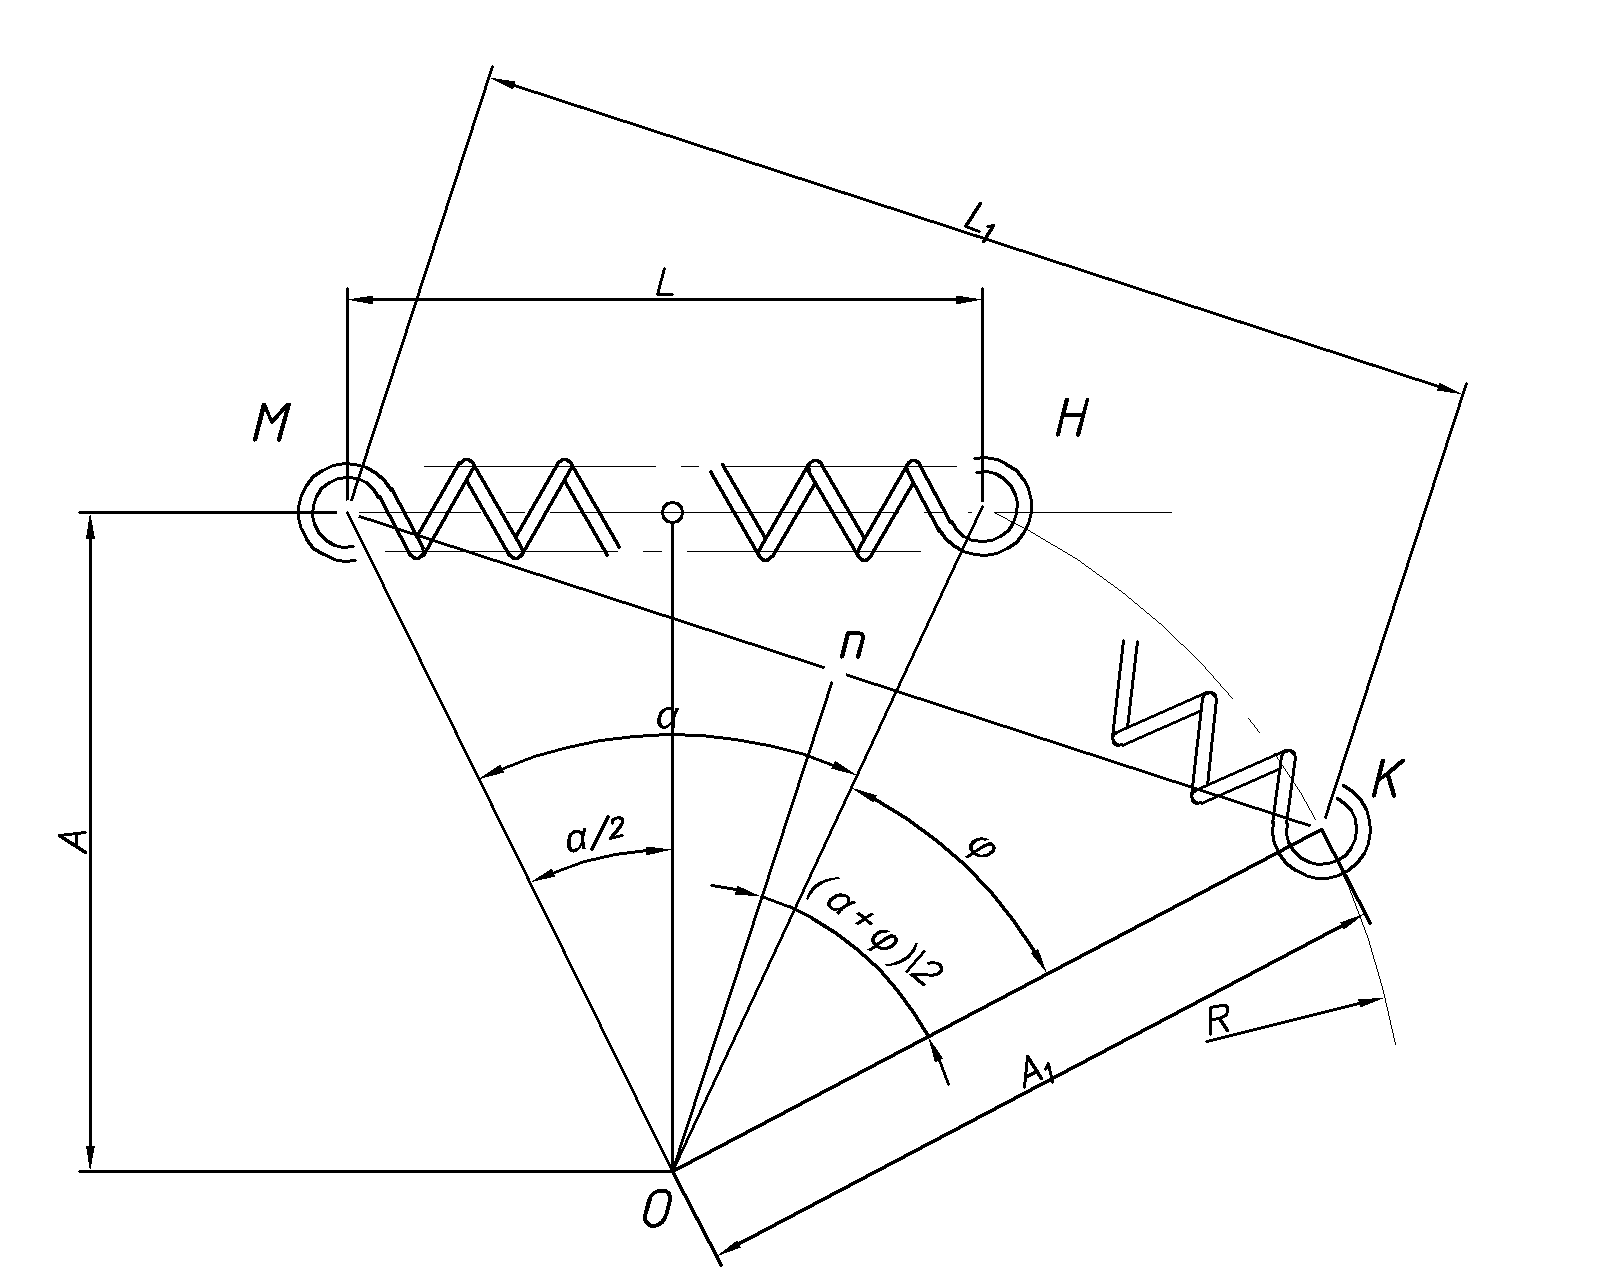
\includegraphics[width=1\linewidth]{loftwheel_shema.png}}
            \caption{К расчёту параметров люфтовыбирающей пружины}
        \end{figure}
        Буквами на рисунке обозначены:
        \begin{table}[h]
            % \begin{left}
                \begin{tabular}{p{0.1\linewidth}p{0.1\linewidth}p{0.8\linewidth}}
                    & L & начальная длина пружины \\
                    & \( L_1 \) & длина пружины в растянутом состоянии \\
                    & \( A \) & начальное плечо \\
                    & \( A_1 \) & новое плечо действия пружины \\
                    & \( \alpha \) & угловой размер пружины в начальном состоянии \\
                    & \( \varphi \) & угол взаимного смещения составных частей колеса \\
                    & \( R \) & расстояние от центра колеса до точки крепления пружины \\
                \end{tabular}
            % \end{left}
        \end{table}
        \\Люфтовыбирающим колесом решено сделать выходное, под номером 10.
        Расчёт пружины ведётся по необходимому рабочему усилию, которое
        вычисляется по формуле [2]:
        \[ P_2 = \frac{\xi M_{\text{кр}}}{2(A\ cos\frac{180^\circ n}{z}
                - \frac{L}{2}\ sin\frac{180^\circ n}{z})},\]
        \begin{table}[h!]
            \begin{center}
                \begin{tabular}{p{0.025\linewidth}p{0.01\linewidth}p{0.8\linewidth}}
                    где & A & - расстояние от оси пружины до центра колеса,\\
                    & n & - число зубьев, на которое производится взаимное смещение составных частей колеса,\\
                    & L & - начальная длина пружины.
                \end{tabular}
            \end{center}
        \end{table}

        Приняв L=¿spr.L¡мм, A=¿loftwheel.A¡мм, n=¿loftwheel.n¡, 
        z=¿loftwheel.z¡, \( \xi=¿loftwheel.xi¡ \), получим:
        \[ P_2 = \frac{¿loftwheel.xi¡\cdot¿loftwheel.M¡}{¿loftwheel.A¡\cdot cos\frac{180^\circ\cdot¿loftwheel.n¡}{¿loftwheel.z¡}
                - \frac{¿spr.L¡}{2}\cdot sin\frac{180^\circ\cdot¿loftwheel.n¡}{¿loftwheel.z¡}} = ¿loft.P2¡\ H\]
        
        Сила пружины при максимальной деформации [2]:
        \[ P_3 = \frac{P_2}{1-\delta} = \frac{¿loft.P2¡}{1-¿loftwheel.d¡} = ¿loft.P3¡\ H\]

        По найденному усилию по таблицам найдём подходящую пружину, склоняясь к более коротким
        и жёстким. Наш выбор: ¿spr.name¡ с параметрами: \( P_3 \) = ¿spr.P3¡ Н, d=¿spr.d¡ мм, 
        D=¿spr.D¡ мм, \( z_1 \)=¿spr.z1¡ Н/мм, \( f_3 \)=¿spr.f3¡ мм. Далее рассчитаем параметры
        пружины для нашего случая.

        Определим величину деформации \( F_2 \) при нагрузке \( P_2 \). Если 
        \[ L_1 =  L\ cos\frac{180^\circ n}{z} + 2A\ sin\frac{180^\circ n}{z} = ¿loft.L1¡\ \text{мм},\]
        то 
        \[ F_2 = L_1 - L = ¿loft.F2¡\ \text{мм}.\]

        Тогда жёсткость определяемой пружины будет
        \[ z = \frac{P_2}{F_2} = \frac{¿loft.P2¡}{¿loft.F2¡} = ¿loft.z¡\ \text{Н/мм}; \]
        необходимое (и полное) число рабочих витков
        \[ n_1 = n = \frac{z_1}{z} = ¿loft.n¡;\]
        длина пружины в свободном состоянии
        \[ H_0 = (n_1 + 1)d = (¿loft.n¡ + 1)\cdot ¿spr.d¡= ¿loft.H0¡\ \text{мм}; \]
        Длина развёрнутой пружины:
        \begin{itemize}
            \item приближённая формула:
                \[ L\approx 3.2Dn_1 = ¿loft.Lapp¡\ \text{мм} \]
            \item точная формула:
                \[ L = \frac{\pi D_0 n}{cos(atan(\frac{d+0.3}{\pi D_0 }))} + \pi D_0 = ¿loft.L¡\ \text{мм};\]
        \end{itemize}
        % \[ L = \frac{\pi D_0 n}{cos(atan(\frac{d+0.3}{\pi D_0 }))} + \pi D_0 = ¿loft.L¡\ \text{мм};\]
        
        полная длина с крючками
        \[ L' = H_0 + 2D = ¿loft.H0¡ + 2\cdot ¿spr.D¡ = ¿loft.L_dash¡\ \text{мм}. \]
        Следовательно, конструктивные размеры выбраны верно.

    \subsubsection{Расчёт валов}
        Рассчитаем предпоследний вал на прочность. 
        \begin{figure}[h]
            \center{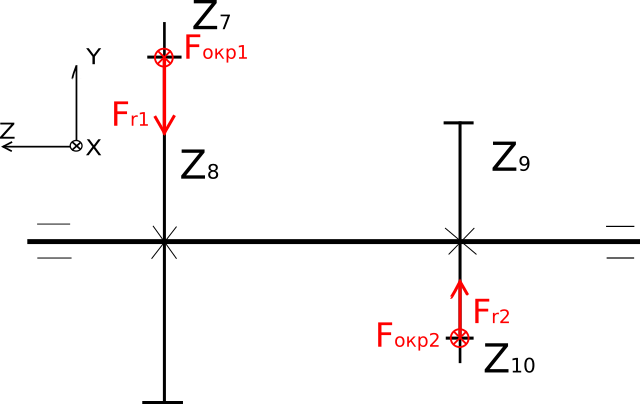
\includegraphics[width=0.7\linewidth]{shaft_schema.png}}
            \caption{Схема вала 4 с приложенными силами}
        \end{figure}
        Найдём необходимые силы (с учётом \( M_4 = ¿shaft.M¡ \)):
        \[ F_{\text{окр1}} = \frac{M_4}{0.5d_1} = ¿shaft.F_circ1¡\ H,\]
        \[ F_{\text{окр2}} = \frac{M_4}{0.5d_2} = ¿shaft.F_circ2¡\ H,\]
        \[ F_{r1} = F_{\text{окр1}}\cdot tan(20^\cdot) = ¿shaft.F_r1¡\ H,\]
        \[ F_{r2} = F_{\text{окр2}}\cdot tan(20^\cdot) = ¿shaft.F_r2¡\ H,\]

        Найдём реакции в опорах.\par
        \begin{figure}[h]
            \center{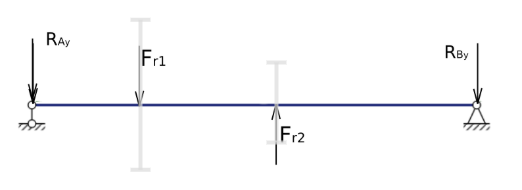
\includegraphics[width=0.8\linewidth]{sh_yoz_2.png}}
            \caption{Схема балки в плоскости YOZ}
        \end{figure}
        \[ \sum M_A = 0 \]
        \[ F_{r_1}\cdot 6 - 15\cdot F_{r_2} + 27\cdot R_{B_y} = 0\]
        \[ R_{B_y} = ¿shaft.R_B_y¡\ H\]
        \[ \sum_{i}^{}F_i = 0 \]
        \[ R_{A_y} + F_{r_1} + R_{B_y} = F_{r_2} \]
        \[ R_{A_y} = ¿shaft.R_A_y¡\ H\]        
        
        \begin{figure}[h]
            \center{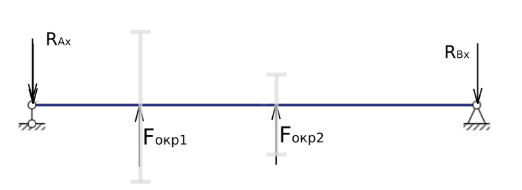
\includegraphics[width=0.8\linewidth]{sh_xoz_2.png}}
            \caption{Схема балки в плоскости XOZ}
        \end{figure}
        \[ \sum M_A = 0 \]
        \[ R_{B_x} = \frac{15\cdot F_{\text{окр2}} + 6\cdot F_{\text{окр1}}}{27} = ¿shaft.R_B_x¡\ H\]
        
        \[ R_{A_x} = F_{\text{окр2}} + F_{\text{окр1}} - R_{B_x} = ¿shaft.R_A_x¡\ H\]

        Представим эпюры рассчитанных моментов:
 
        \begin{figure}[!h]
            \center{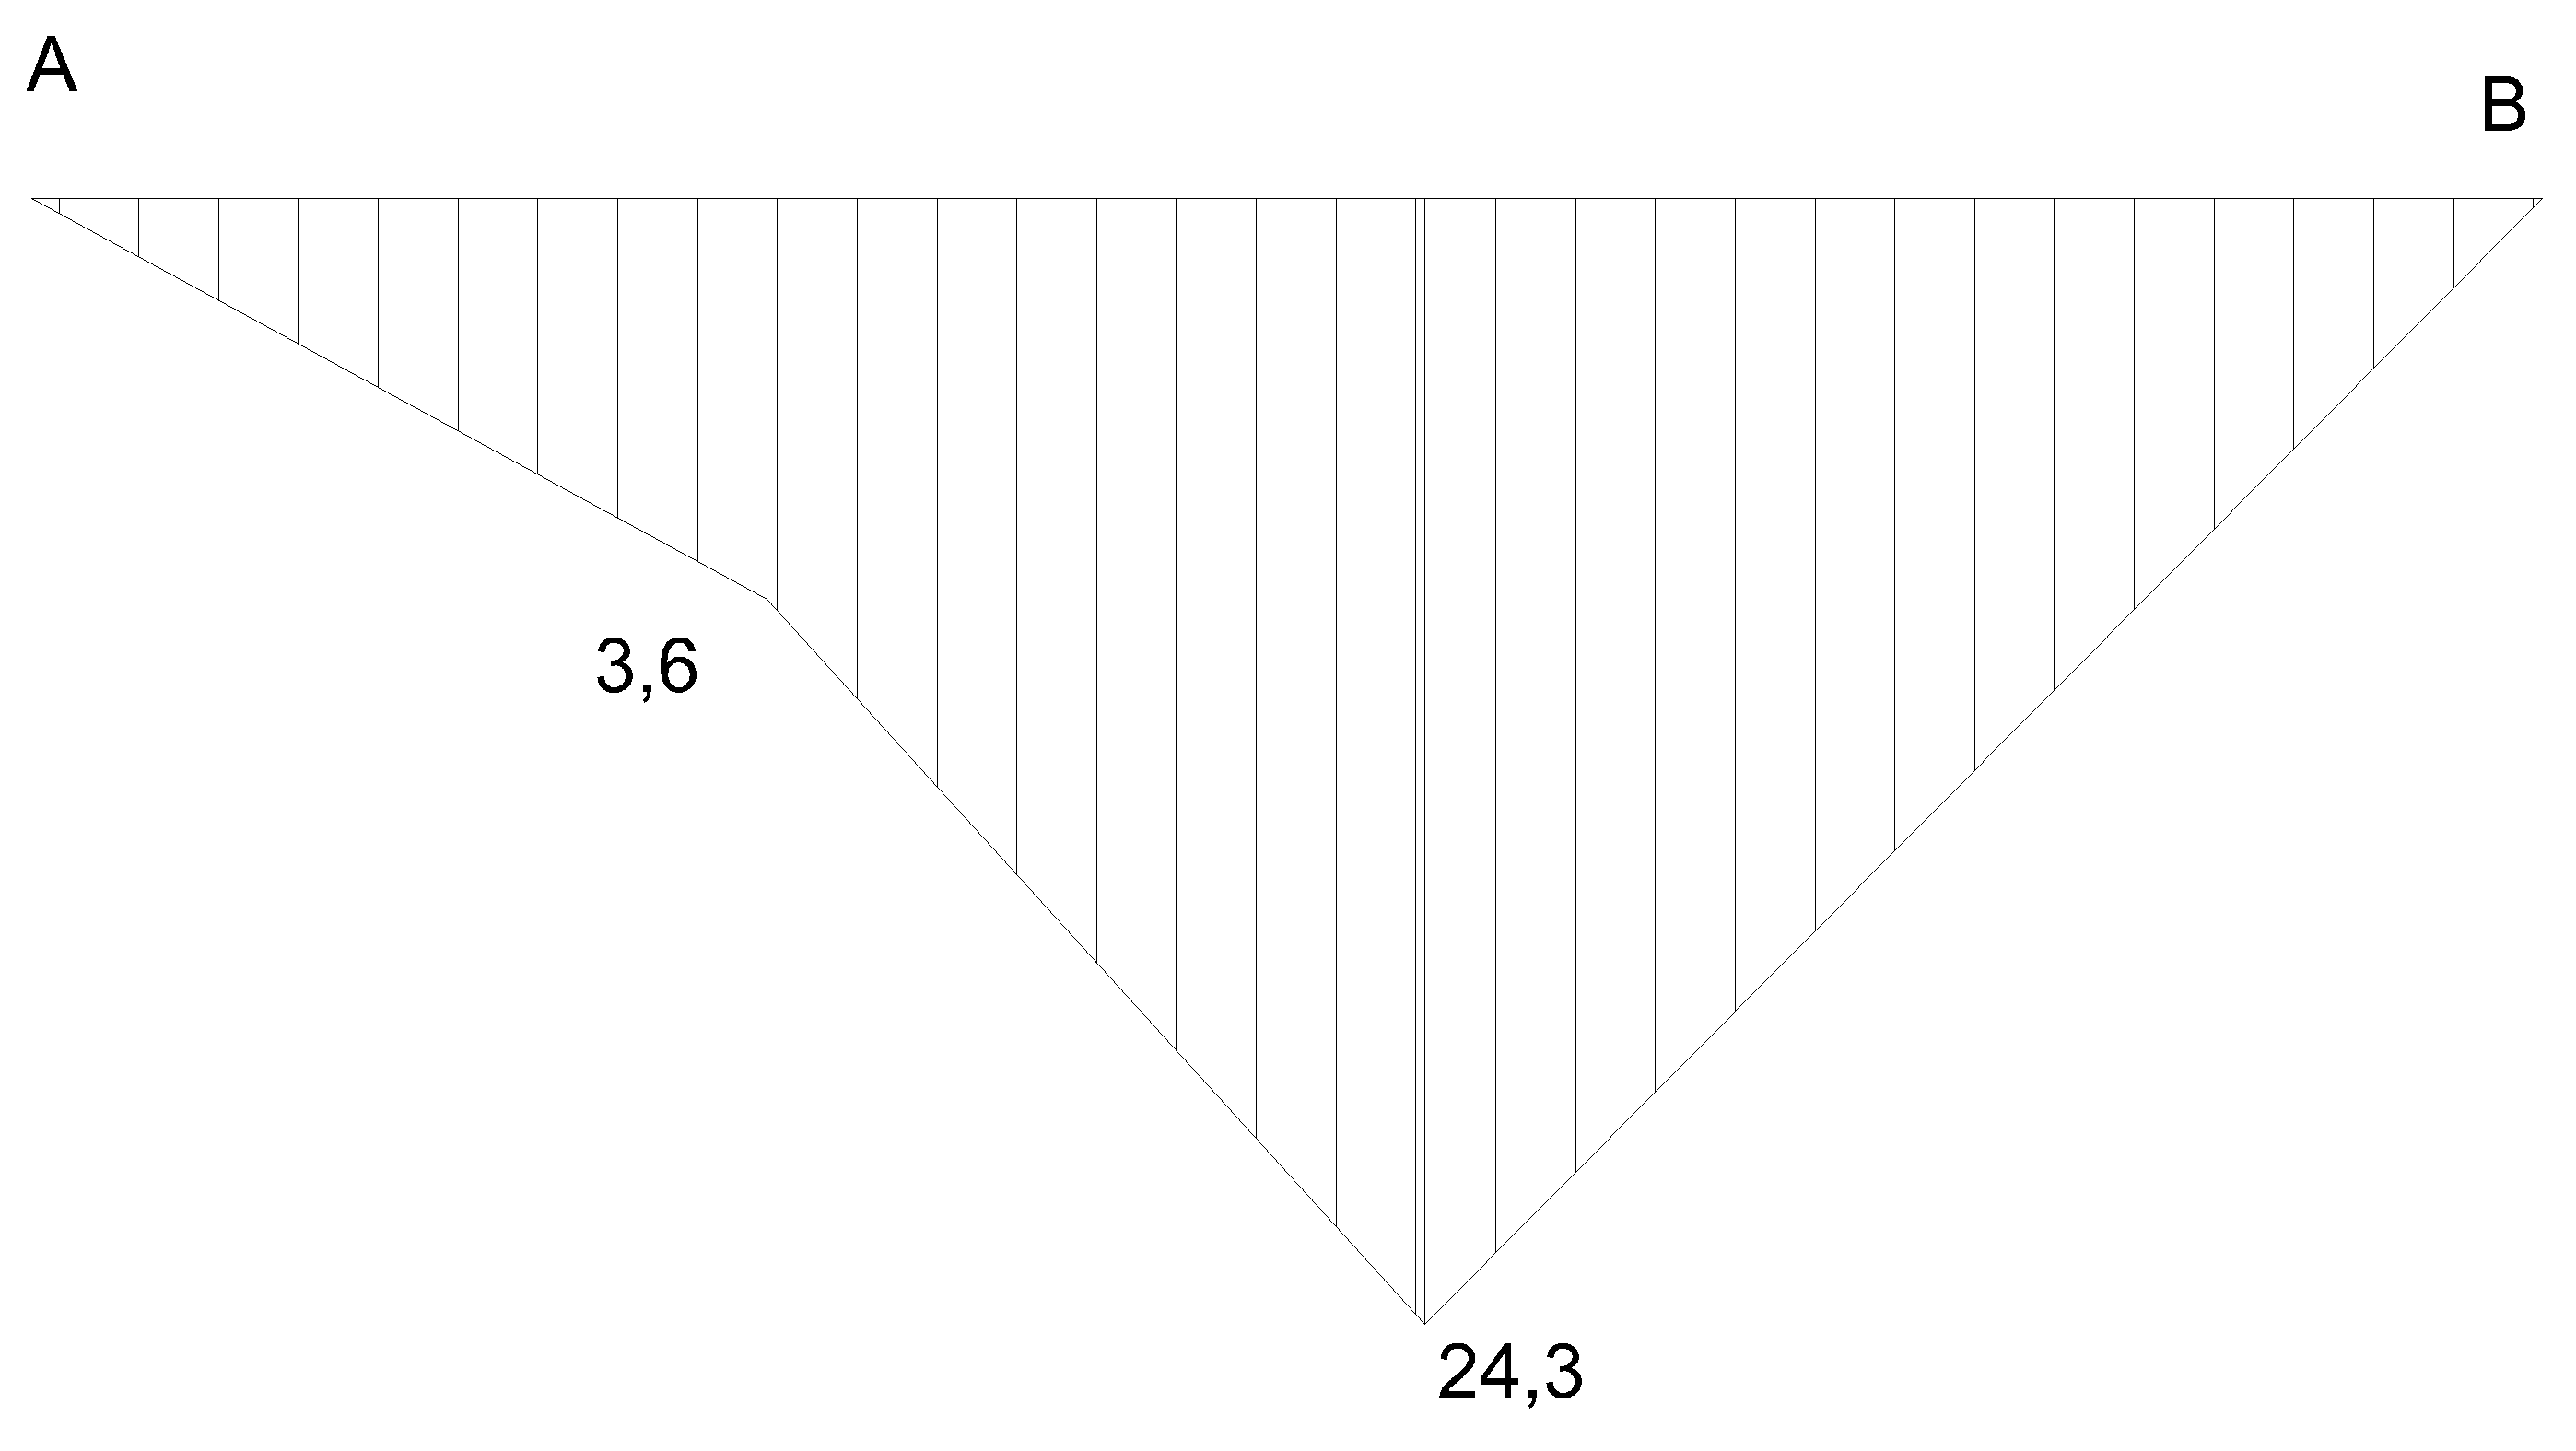
\includegraphics[width=0.8\linewidth]{epure_yoz.png}}
            \caption{Эпюра изгибающего момента в плоскости YOZ}
        \end{figure}

        \begin{figure}[h]
            \center{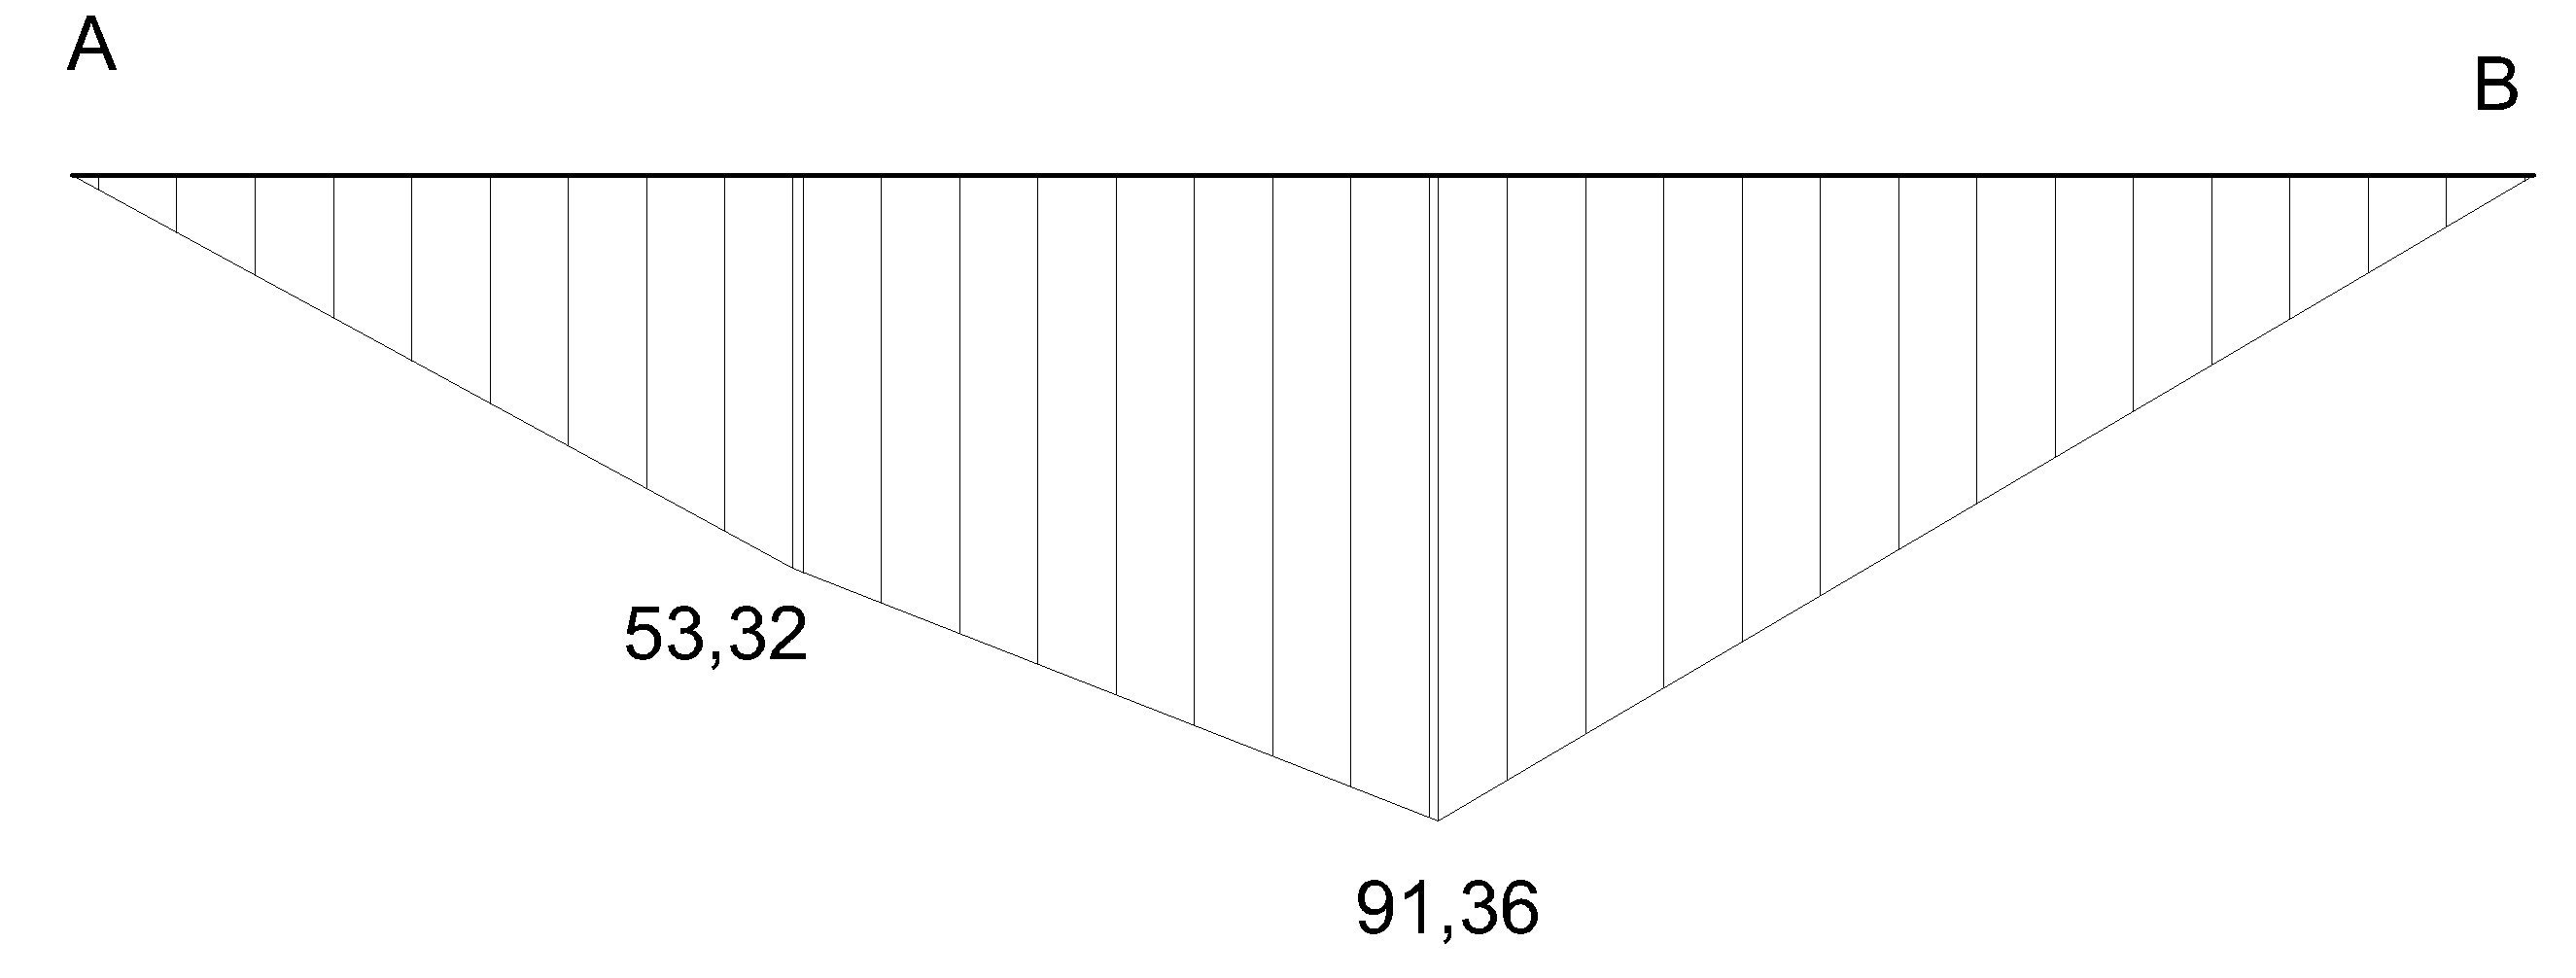
\includegraphics[width=0.8\linewidth]{epure_xoz.png}}
            \caption{Эпюра изгибающего момента в плоскости XOZ}
        \end{figure}
        \begin{figure}[h]
            \center{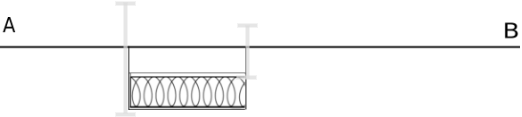
\includegraphics[width=0.8\linewidth]{epure_circ_2.png}}
            \caption{Эпюра крутящего момента}
        \end{figure}

        Учтя, что на вал действуют одноврененно и изгибающий, и крутящий моменты,
        проведём расчет на прочность через приведенный момент в опасном сечении.
        По эпюрам очевидно, что это сечение находится на месте крепления шестерни
        (зубчатого колеса №9).

        \[ M^{\sum}_\text{изг} = \sqrt{M_x^2 + M_y^2} = \sqrt{¿shaft.Mkx¡^2 + ¿shaft.Mky¡^2} = ¿shaft.Msum_izg¡\ \text{Нмм}\]
        \[ M_\text{прив.} = \sqrt{{M^{\sum}_\text{изг}}^2 + 0,75M_\text{кр}^2} = ¿shaft.M_pr¡\ \text{Нмм}\]

        Расчёт минимального диаметра вала проведём по формуле [1]:
        \[ d\geq \sqrt[3]{\frac{M_\text{пр}}{0,1[\sigma_F]}}, \]
        где \( [\sigma_F] \) - допускаемое изгибающее напряжение, вычисляется как
         \( [\sigma_F] = 0,1[\sigma_b] \).\par
        Материалом выберем сталь 40Х, параметры которой приведены в таблице \ref{tab:gear_materials}.\par

        \[ d\geq \sqrt[3]{\frac{¿shaft.M_pr¡}{0,1\cdot 0,1\cdot ¿material.s.sigma_b¡}} = ¿shaft.d_min¡\ \text{мм} \]
        Принимаем минимальный диаметр ближайшим сверху из стандартных диаметров, равным
        \( d_{\text{мин}} = 3\ \text{мм} \), который при этом вполне подходит по конструктивным
        соображениям. Такой диаметр будет у вала в местах крепления к подшипникам.

    \subsubsection{Расчёт штифтов}
        Расчитаем минимальный диаметр штифта. Для этого воспользуемся следующей формулой:
        \[ d_\text{ш} \geq 2\sqrt{\frac{M}{\pi d [\tau_{\text{ср}}]}}, \]
        где \( [\tau_{\text{ср}}] \) - допустимое напряжение на срез, МПа,\\
        \( d \) - диаметр вала, мм,\\
        \( M \) - крутящий момент на валу, Нмм.
        Материалом для штифта примем Сталь50, для неё \( [\tau_{\text{ср}}] =75\) МПа.
        Так как все валы в местах посадки зубчатых колёс имеют одинаковую толщину d=4мм, то рассчитаем
        толщину штифта для наиболее нагруженного вала V.
        \[ d_\text{ш} \geq 2\sqrt{\frac{¿M4¡}{\pi\cdot 4\cdot 75}} = 0,72\ \text{мм} \]
        Округлив в большую сторону, примем диаметром штифтов \( d_\text{ш} = 1 \) мм.
        

    \subsubsection{Расчёт опор}
        Подберём опоры для валов. Выберем опоры качения, а именно - радиальные подшипники,
        так как нагрузка на валы только радиальная.\par
        Применем формулу для расчёта динамической грузоподьемности [1] (т.к. скорость вращения
        больше 1 об/мин):
        \[ C_P = 0,01P\sqrt[3]{60nL_h}, \]
        где n - частота вращения рассчитываемого вала (IV), об/мин, \\P - эквивалентная
        динамическая нагрузка,\\ \( L_h \) - время работы, ч.\par
        Рассчитаем P по формуле [1]:
        \[ P = (XF_r + YF_a)k_\sigma k_\tau = ¿shaft.P¡\ H, \]
        где (X, Y) = (1, 0) - коэффициенты, учитывающие направление нагрузки,\par
            \( k_\sigma = 1 \) - коэффициент безопасности,\par
            \( k_\tau=1,2 \) - коэффициент температуры,\par
            \( F_r \) - радиальная нагрузка, \par
            \( F_a \) - осевая нагрузка (равна 0).\par
        Приняв n=218 об/мин, \( L_h \) = 3000ч, получаем
        \[ C_P = 0,01\cdot ¿shaft.P¡ \cdot \sqrt[3]{60\cdot ¿shaft.n¡\cdot 3000} = ¿shaft.Cp¡\ H \]
        \cite{Dorf}
        На основе полученного значения выберем подшипник "¿podsh.name¡" со следующими
        параметрами:
        \begin{table}[h!]
            \begin{center}
                \begin{tabular}{p{0.13\linewidth}p{0.13\linewidth}p{0.13\linewidth}p{0.13\linewidth}p{0.13\linewidth}p{0.13\linewidth}}
                    \hline
                    d, \( \text{мм} \) & D, \( \text{мм} \) & B, \( \text{мм} \) & r, \( \text{мм} \) & C, Н & \( C_0 \), Н \\
                    \hline
                    ¿podsh.d¡ & ¿podsh.D¡ & ¿podsh.B¡ & ¿podsh.r¡ & ¿podsh.C¡ & ¿podsh.C0¡ \\
                    \hline
                \end{tabular}
                \caption{{Характеристики основного подшипника}}\label{tab:podsh}
            \end{center}
        \end{table}

        Выберем такой подшипник для всех валов.

    
\subsection{Расчёт показателей точности кинематической схемы}
    \subsubsection{Расчёт погрешности}
        Для зубчатой передачи назначим 7-ю степень точности как 
        наиболее часто применяемую для точных передач. Кроме того, приняв во 
        внимание окружные скорости колёс, возможное изменение размеров
        из-за колебаний температуры и прочие параметры, назначаем
        для передач сопряжение F.\par

        Общую погрешность передачи находят находят как сумму люфтовой и
        кинематической погрешностей:
        \[ \Delta\varphi_{\sum} = \Delta\varphi_{i0}  + \Delta\varphi_{\text{л}}\]
        
        Рассчитаем люфтовую погрешность. Она складывается из погрешностей
        элементарных передач \( \Delta\varphi_{\text{л}i} \), нормированных
        на соответствующее передаточное отношение. \par 

        Значение погрешностей для цилиндрических передач определяют в
         угловых минутах по формуле:
         \[ \Delta\varphi_{\text{л}i} = 7,4\frac{j_{n-max}}{mz}, \]
         где\par \qquad m - модуль колеса, мм;\par
            \qquad\( z \) - число зубьев колеса\par
            \qquad\( j_{n-max} \) - вероятный максимальный угловой зазор, мкм.\par
        
        С учётом типа сопряжения возьмём из ГОСТ 9178-81 значения \( j_{n-max} \)   :
        \begin{table}[h!]
            \begin{center}
                \begin{tabular}{p{0.15\linewidth}|p{0.17\linewidth}p{0.17\linewidth}p{0.17\linewidth}p{0.17\linewidth}p{0.17\linewidth}}
                    \hline
                    \( a_w \), мм & ¿gears.1.a¡ & ¿gears.3.a¡ & ¿gears.5.a¡ & ¿gears.7.a¡ & ¿gears.9.a¡ \\
                    \hline
                    \( j_{n max} \), мкм & 11 & 11 & 13 & 16 & 19 \\
                    \hline
                \end{tabular}
            \end{center}
        \end{table}

        Вычислим погрешности:
        \[ \Delta\varphi_{\text{л}12} = 7.4\frac{11}{¿gears.1.m¡\cdot ¿gears.1.z¡} = ¿acc.0.phi_L¡' \]
        \[ \Delta\varphi_{\text{л}34} = 7.4\frac{11}{¿gears.3.m¡\cdot ¿gears.3.z¡} = ¿acc.1.phi_L¡' \]
        \[ \Delta\varphi_{\text{л}56} = 7.4\frac{13}{¿gears.5.m¡\cdot ¿gears.5.z¡} = ¿acc.2.phi_L¡' \]
        \[ \Delta\varphi_{\text{л}78} = 7.4\frac{16}{¿gears.7.m¡\cdot ¿gears.7.z¡} = ¿acc.3.phi_L¡' \]
        \[ \Delta\varphi_{\text{л}9\ 10} = 7.4\frac{19}{¿gears.9.m¡\cdot ¿gears.9.z¡} = ¿acc.4.phi_L¡' \]
        
        Соответственно, люфтовая погрешность равна:
        \[ \Delta\varphi_{\text{л}} = \sum_{k=1}^{5}\frac{\Delta\varphi_{\text{л}k}}{i_{k-n}} = ¿acc.phi_L¡'\]
        
        Рассчитаем кинематическую погрешность, приведённую к выходному валу. Она складывается из погрешностей
        элементарных передач \( \Delta\varphi_{\text{i}k} \) по следующей формуле:
        \[ \Delta\varphi_{i0} = \frac{\Delta\varphi_{i1}}{i_{1-(n+1)}} +  
        \frac{\Delta\varphi_{i2}+\Delta\varphi_{i3}}{i_{2-(n+1)}} + ... + \Delta\varphi_{i2n} \]

        Величина \( \Delta\varphi_{i} \) определяется по формуле:
        \[ \Delta\varphi_{i} = 4.8\frac{F_p+F_f}{mz}, \]
        где\par
            \qquad\( F_p \) - допуск на накопленную погрешность шага зубчатого колеса,мкм;\par
            \qquad\( F_f \) - допуск на погрешность профиля зуба, мкм;\par
        
        По ГОСТ 9178-81 найдём эти погрешности и рассчитаем погрешности:
        
        \begin{table}[h!]
            \begin{center}
                \begin{tabular}{p{0.1\linewidth}|p{0.07\linewidth}p{0.07\linewidth}p{0.07\linewidth}p{0.07\linewidth}p{0.07\linewidth}p{0.07\linewidth}p{0.07\linewidth}p{0.07\linewidth}p{0.07\linewidth}p{0.07\linewidth}}
                    \hline
                    m, мм  & \multicolumn{2}{c}{¿gears.1.m¡} & \multicolumn{2}{c}{¿gears.3.m¡} & \multicolumn{2}{c}{¿gears.5.m¡} & \multicolumn{2}{c}{¿gears.7.m¡} & \multicolumn{2}{c}{¿gears.9.m¡} \\
                    z       & ¿gears.1.z¡ &  ¿gears.2.z¡ &  ¿gears.3.z¡ &  ¿gears.4.z¡ &  ¿gears.5.z¡ & ¿gears.8.z¡ &   ¿gears.7.z¡ &  ¿gears.8.z¡ &  ¿gears.9.z¡ &  ¿gears.10.z¡ \\
                    d, мм   & ¿gears.1.d¡ &  ¿gears.2.d¡ &  ¿gears.3.d¡ &  ¿gears.4.d¡ &  ¿gears.5.d¡ & ¿gears.6.d¡ &   ¿gears.7.d¡ &  ¿gears.8.d¡ &  ¿gears.9.d¡ &  ¿gears.10.d¡ \\
                    \( F_P \), мкм & 22 & 24 & 22 & 24 & 22 & 30 & 22 & 35 & 26 & 42 \\
                    \( F_f \), мкм & 9 & 9 & 9 & 9 & 9 & 9 & 9 & 9 & 10 & 10 \\
                    \( \Delta\varphi_{i},  \) угл. мин. & ¿acc.1.phi_i¡ & ¿acc.2.phi_i¡ & ¿acc.3.phi_i¡ & ¿acc.4.phi_i¡ & ¿acc.5.phi_i¡ & ¿acc.6.phi_i¡ & ¿acc.7.phi_i¡ & ¿acc.8.phi_i¡ & ¿acc.9.phi_i¡ & ¿acc.10.phi_i¡ \\
                    i  & \multicolumn{2}{c}{¿gears.1.i¡} & \multicolumn{2}{c}{¿gears.3.i¡} & \multicolumn{2}{c}{¿gears.5.i¡} & \multicolumn{2}{c}{¿gears.7.i¡} & \multicolumn{2}{c}{¿gears.9.i¡} \\
                    \hline
                \end{tabular}
                \caption{{Характеристики зубчатых колес}}\label{tab:gears_digest}
            \end{center}
        \end{table}

        Тогда общая кинематическая погрешность равна:
        \[ \Delta\varphi_{i0} = 
                \frac{¿acc.1.phi_i¡}{¿acc.I_mul.0¡}
                + \frac{¿acc.2.phi_i¡+¿acc.3.phi_i¡}{¿acc.I_mul.1¡}
                + \frac{¿acc.4.phi_i¡+¿acc.5.phi_i¡}{¿acc.I_mul.2¡}+\]
              \[+ \frac{¿acc.6.phi_i¡+¿acc.7.phi_i¡}{¿acc.I_mul.3¡}
                + \frac{¿acc.8.phi_i¡+¿acc.9.phi_i¡}{¿acc.I_mul.4¡}
                + ¿acc.10.phi_i¡ = ¿acc.Phi¡'\]
        
        А суммарная погрешность:
        \[ \Delta\varphi_{\sum} = \Delta\varphi_{i0}  + \Delta\varphi_{\text{л}} 
        = ¿acc.Phi_l¡ + ¿acc.Phi¡ = ¿acc.Sum¡' \]
        
        
        

        
        
        
        
        
        
        
        

        
        
\newpage
        ferefr
\renewcommand\refname{Список использованных источников}
\addcontentsline{toc}{section}{4. Список использованных источников}
\bibliographystyle{utf8gost705u}  %% стилевой файл для оформления по ГОСТу
\bibliography{biblio}
        
[1] Тищенко \par
[2] Шарловский
    
\end{document}